\documentclass[12pt, letterpaper]{article}
\usepackage[
    backend=biber,
    style=alphabetic,
]{biblatex}
\usepackage{graphicx}
\graphicspath{{diagrams/}}
\addbibresource{sources.bib}

\title{\Huge \textbf{Software-Implemented Fault Tolerance}}
\author{Filip Ďuriš}

\begin{document}

\maketitle

\newpage

\begin{abstract}
With the increasing demand for high-performance embedded software comes the inevitable, difficult task of ensuring fault-free functioning of ever-more complex systems. The increased complexity, both in terms of hardware components and software features, increases the number of failure points where errors can occur.

Errors can be caused by both external factors beyond our control such as radiation in space, but also as a result of human error while designing the software. Due to the incredibly complex nature of this problem, it is unlikely that we will be designing completely error-free software and hardware in the near future. This simple fact makes fault-tolerance an important aspect of software design, especially when designing critical systems whose failure could endanger human life. However, as with most things, fault-tolerance and reliability is a trade-off, which usually comes at the cost of performance, development time and cost.

This paper will aim to analyze various commonly implemented fault-tolerance methods. We will look at the benefits and drawbacks of the utilized methods, as well as construct a working demo based on FreeRTOS that implements and tests the effectiveness of some selected methods.
\end{abstract}



\section{Taxonomy}

For the sake of consistency in the nomenclature used in this paper, we will refer to the naming conventions and definitions as outlined in \cite{1335465}. Below is a listing of the most crucial terms used in this paper and their definitions.

\subsection{Failure}
Failure is an event that occurs when the delivered service deviates from correct service. A service fails either because it does not comply with the functional specification, or because this specification did not adequately describe the system function. A service failure is a transition from correct service to incorrect service, i.e., to not implementing the system function. 

\subsection{Error}
Error is a deviation of the service from its correct state. It is a part of the system's state that may lead to service failure. Errors are the result of issues within the software, an example might be the lack of input sanitization, possibly leading to unexpected values as input.

\subsection{Fault}
Fault is the actual or hypothesized cause of a error. Faults are usually considered dormant until manifested, causing an error. An example of a fault might be hardware issue causing an I/O device to send corrupted data as input. If the software is not designed to deal with incorrect input this would lead to an internal error, possibly causing a service failure.

Faults can be further split into various categories, the ones mostly relevant to use are **external faults** which originate from outside the system boundaries and propagate into the system. Which also includes **natural faults** that are caused by natural phenomena without human particiaption. These faults can the hardware and the software, which is why we can further classify them as **hardware faults** and **software faults**.

\subsection{Fault tolerance}
Is the ability to avoid service failures in the presence of faults.

\section{Types of faults}

Errors can be caused by numerous factors, some of which are under the control of developers and some which are not. Generally speaking, we can split errors into two categories - hardware errors - these are predominantly out of our control as developers, and software errors - these errors are usually within our control, but due to various factors are still an important consideration when designing software.

\subsection{Hardware faults}

Hardware errors are caused by external factors beyond our control as software developers. They are usually caused by environmental influences, such as cosmic radiation in space, electro-magnetic fields or adverse weater conditions. In order to create robust and reliable software, which can continue operation even when hardware errors do occur, we must implement software redundancies which maximize the likelyhood of the software executing correctly under all conditions.

One of the most common hardware errors is memory corruption, which can appear in many forms and result from a wide range of causes. For instance, radiation exposure in space can cause single-event upsets (SEUs), flipping individual bits in memory and altering data unpredictably. Similarly, physical damage to storage media, such as hard drives or SSDs, might corrupt specific regions of the file system, making certain data inaccessible or incorrect.

Memory corruption is not always catastrophic. While it can result in complete system failure and unrecoverable states, it is just as likely to manifest as small, hard-to-detect errors. These subtle corruptions might not immediately disrupt the software's functioning but can lead to unpredictable behavior over time.

A defining characteristic of hardware errors, including memory corruption, is their unpredictability. This makes it essential to implement robust fault-tolerance strategies, such as error detection and correction codes (ECC) in memory, periodic integrity checks, and recovery mechanisms to verify and restore corrupted states. These measures ensure that systems remain operational even when errors occur, minimizing the impact of hardware faults on overall reliability.

\subsection{Development faults}

Software faults, introduced during the development process, are considered development faults. These errors are typically caused by improper handling of user inputs, faulty logic, or inadequate resource management, among other issues. Recognizing that software will likely contain bugs, regardless of how much effort we put into it, is essential to creating resilient and fault-tolerant applications. Accepting the inevitability of bugs allows developers to incorporate strategies for managing potential failures.

To ensure that software remains robust and as free of errors as possible, there are several effective strategies. One promising approach we will look at is the use of memory-safe programming languages, specifically Rust. Rust is a modern language that has gained traction for its safety features, particularly in system programming and embedded applications. It ensures high performance through zero-cost abstractions and introduces a memory ownership model, which reduces memory-related errors such as null pointer dereferencing and data races. This model makes Rust particularly well-suited for low-level and resource-constrained environments, where reliable memory management is crucial. (https://docs.rust-embedded.org/book/)

\section{Fault tolerant software}

\subsection{Single version vs multi-version}

\subsection{Single version}

Single version is a technique which focuses on creating a singular, robust implementation of software by integrating safety checks and redundancies directly into its design. The primary aim of this approach is to make the software as resilient as possible to errors and external factors, ensuring reliable operation under a wide range of conditions.

This technique emphasizes the detection of faults within the software and the ability to recover from them. Fault detection typically involves monitoring the system for unexpected behaviors or inconsistencies, which could signal the presence of an error. Recovery mechanisms then act to mitigate the effects of these faults, either by correcting them or transitioning the system into a stable, functional state.

Drawbacks of single version techniques are primarily the lack of alternatives and fallbacks, should the version fail. Single-version techniques heavily rely on error detection and recovery, which might not always work in practise.

\subsubsection{Modularity}

Perhaps the simplest way we can create a more resilient software is to structure it into independed modules. Each module should handle one task and, when possible, not directly rely upon any other modules for its functionality, or be relied upon by other modules.

A technique commonly utilized to achieve modularity is partitioning, which can be divided into horizonatal and vertical partitioning. Horizontal partitioning aims to split the software into independent structural branches communicating through interfaces. 
Vertical partitioning splits the software in a top-down fashion, where higher level modules are tasked with control logic while lower level modules do most of the processing (https://ntrs.nasa.gov/api/citations/20000120144/downloads/20000120144.pdf).

\begin{figure}[hbt!]
    \centering
    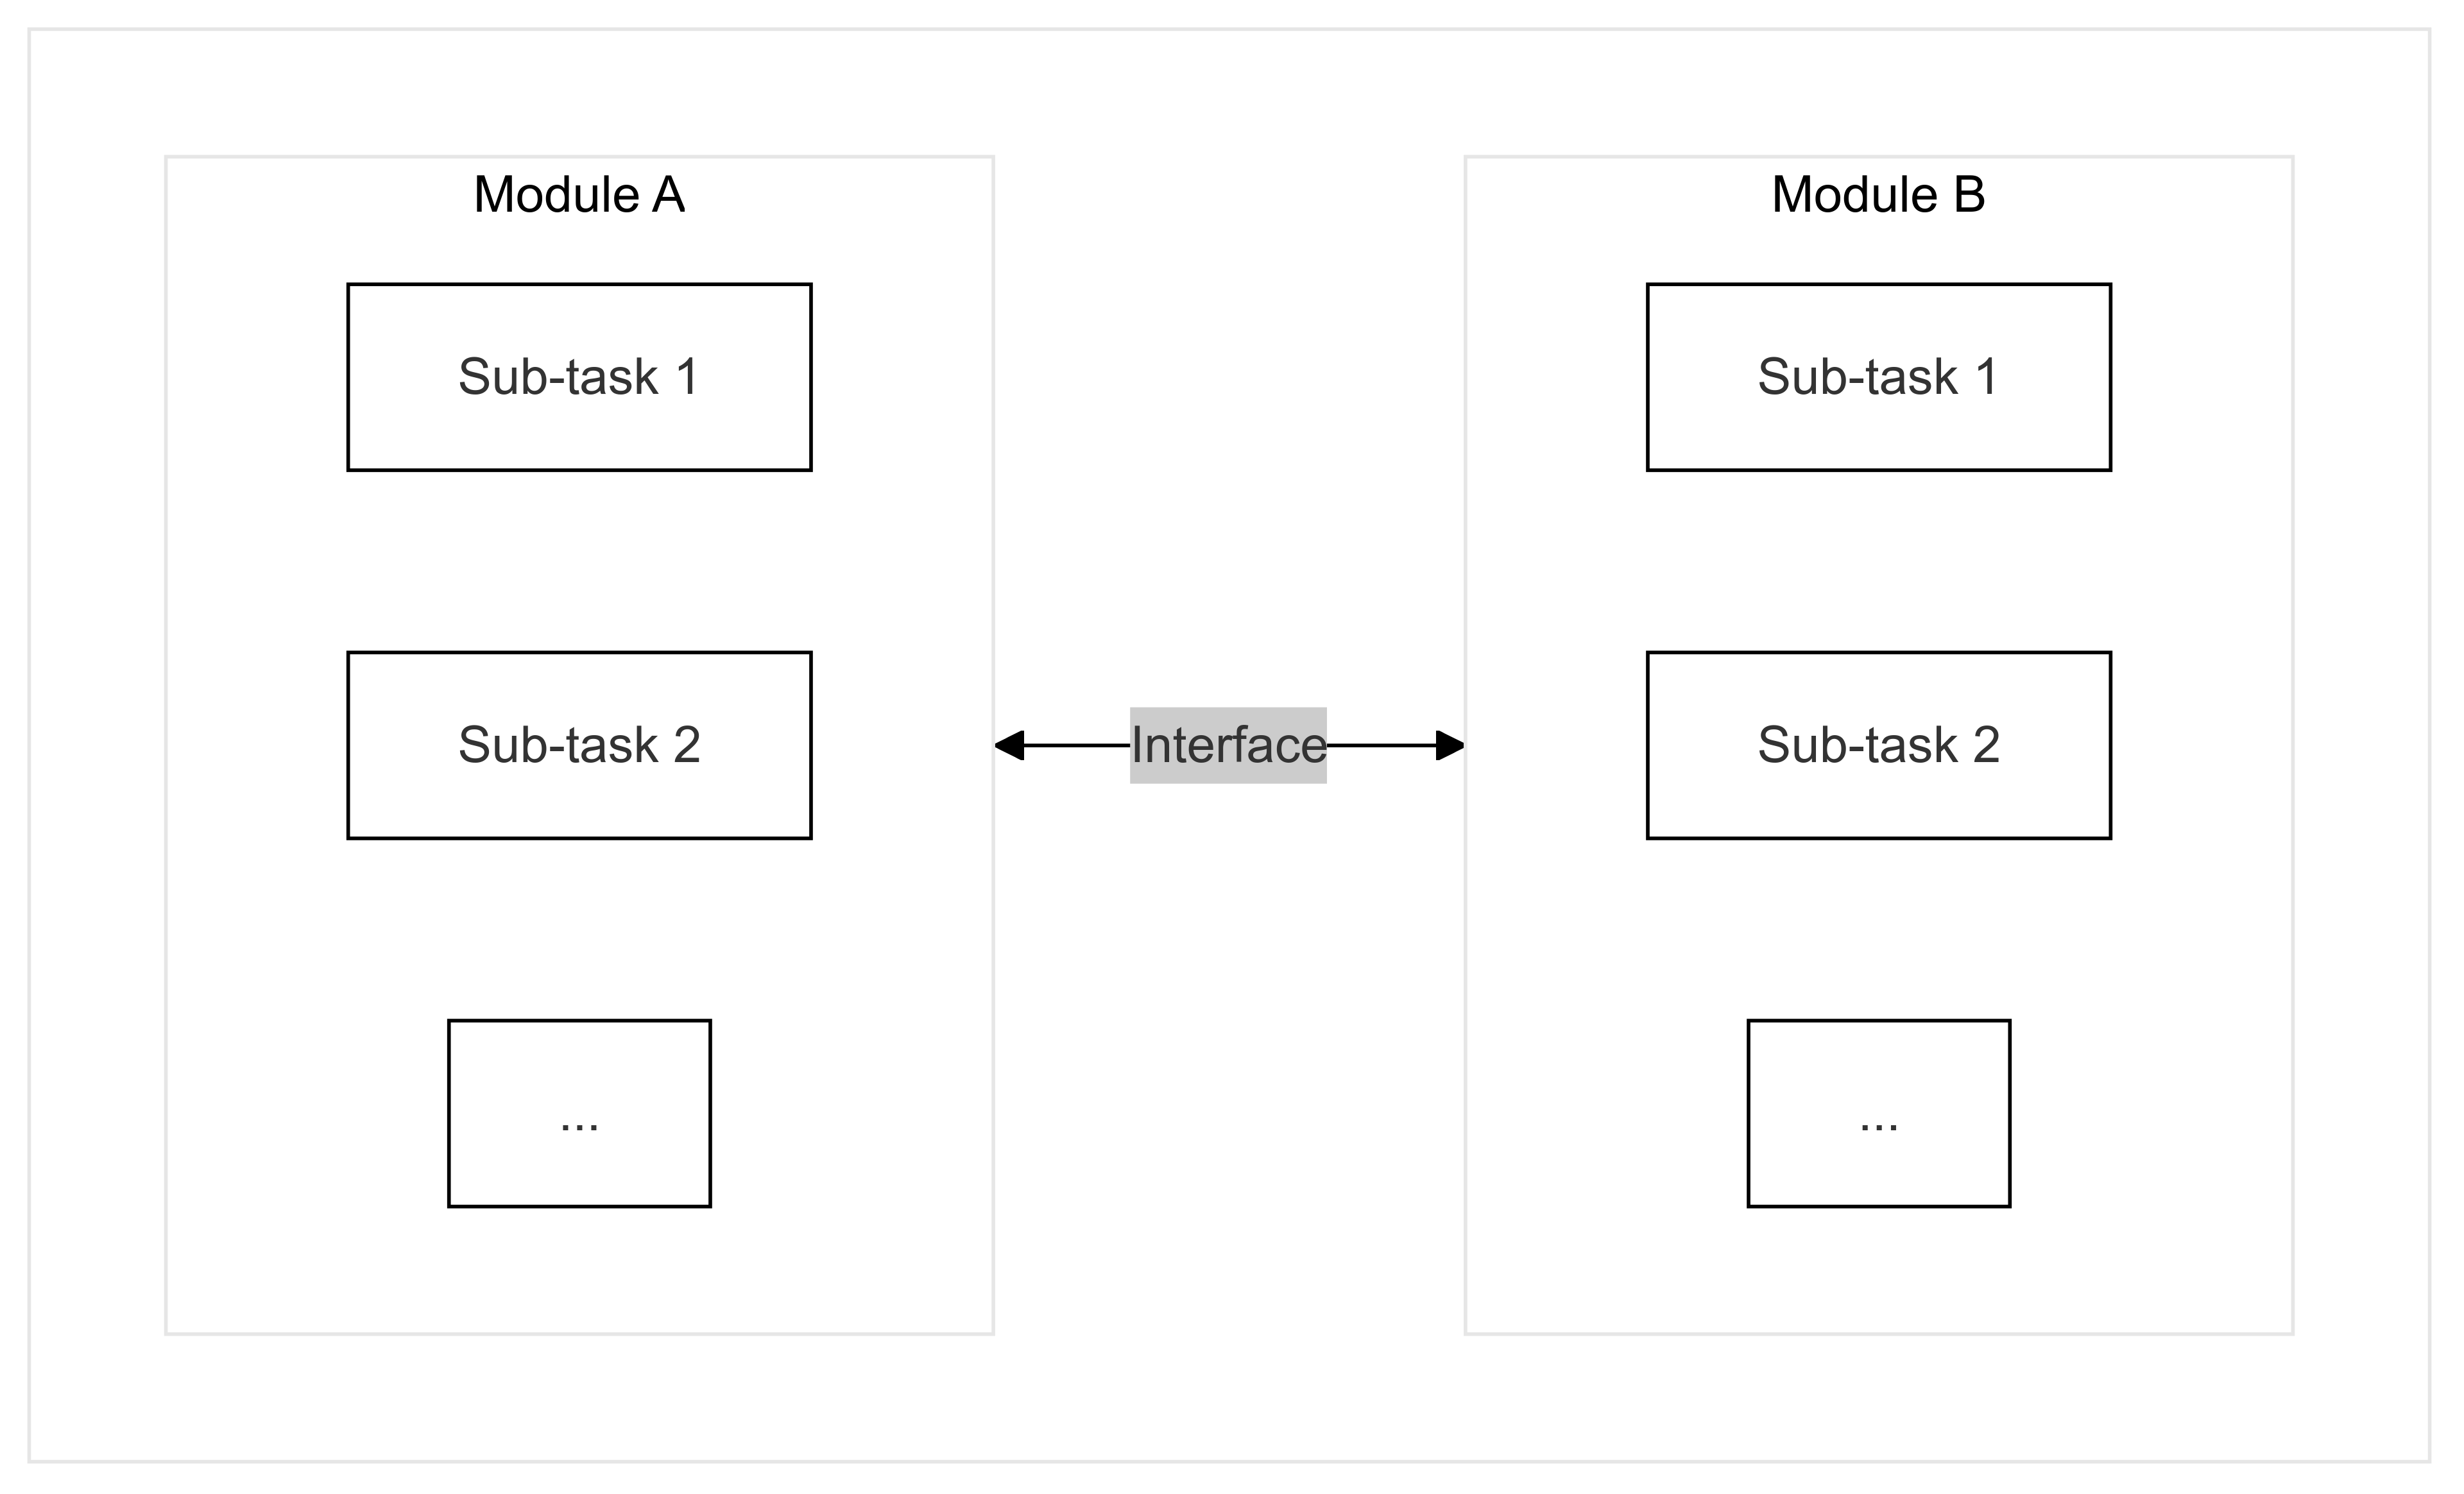
\includegraphics[width=0.7\textwidth]{modularity/horizontal.png}
    \caption{Horizontal partitioning}
    \label{fig:mod_hor}
\end{figure}

\begin{figure}[hbt!]
    \centering
    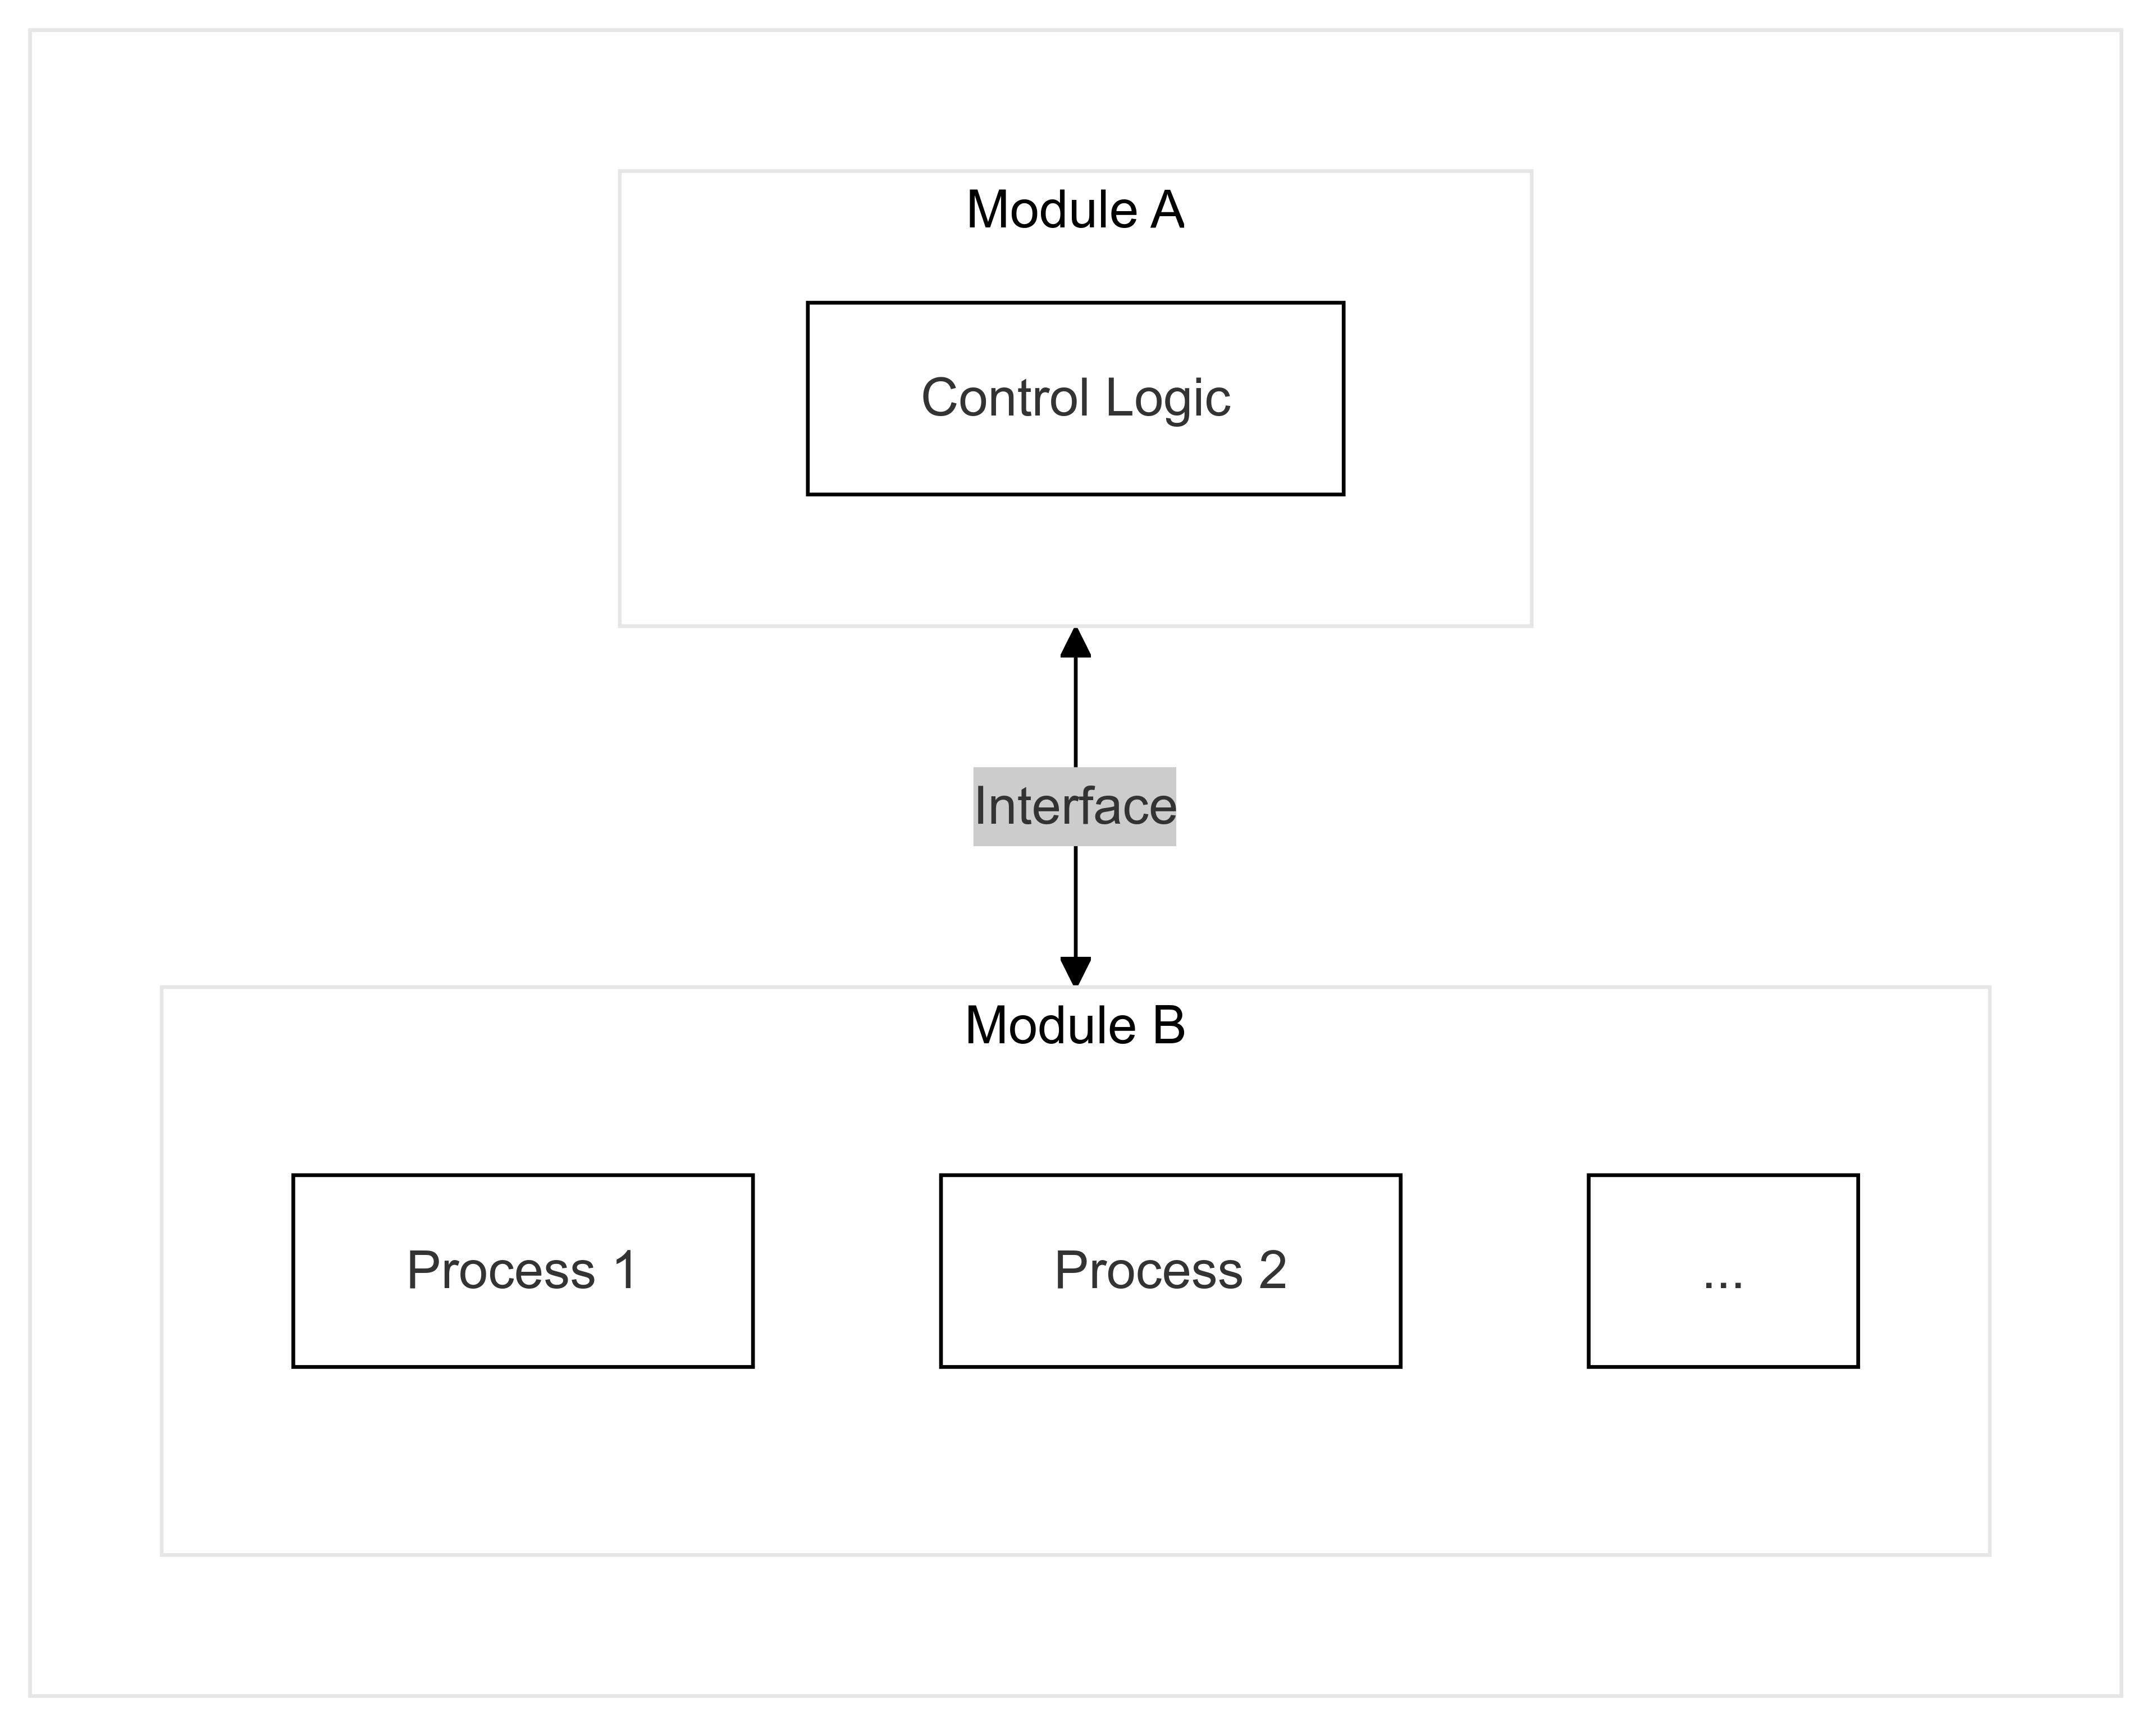
\includegraphics[width=0.7\textwidth]{modularity/vertical.png}
    \caption{Vertical partitioning}
    \label{fig:mod_ver}
\end{figure}

Benefit of partitioning is the ability of software to isolate errors. Provided the sofware is correctly structured, an error occuring in a single module should not propagate to other modules. Meaning we can use modularity as a way to pinpoint the erroneous parts of software and attempt recovery. If recovery is not possible, the software should still be able to partially function, given that other parts of the software are not influenced by the fault. In most situations, partial functioning of a software is preferrable to a complete shutdown.

\subsubsection{Error detection}

Fault-tolerant single-version application should meet two main criteria: self-protection and self-checking. Self-protection means that the application should be able to protect itself from external corruption by detecting errors in information being passed into the application. Self-checking means that the application component must be able to detect errors within itself and prevent propagation of these errors into other components. These two traits combined can be together considered as the ability of "error detection".
(https://ntrs.nasa.gov/api/citations/20000120144/downloads/20000120144.pdf)

Error detection covers a wide range of techniques used to locate errors and mittigate them. Some common approaches include:

a) checksums and error correction codes (ECC), which embed additional metadata with the actual data in order to verify integrity and attempt to correct corrupted data. This approach allows for some degree of memory corruption mitigation but comes at the cost of memory overhead and additional processing per data-chunk which uses checksum or ECCs.

b) assertion and runtime checks, which perform independent checks on the data during execution which ensures the data matches the expected outcomes at certain checkpoints. This approach also carries with it the additional processing overhead without guarantees that we will be able to catch all errors.

c) watchdog timers, whose main purpose is to catch deadlock states by giving a task a certain amount of time to exectue before aborting it.

Error detection is a crucial aspect of single-version application, since we have no alternate version to fall back upon (see section 3).

\subsubsection{Exception handling}

\subsubsection{Checkpoint and restart}

\subsection{Multi-version}

Multi-version relies on multiple different version of the same software, where the failure of a single variant does not have an impact on the overall system.
Multiple versions of the same software are exectues either in sequence or in parallel, each utilizing different error detection and recovery, to have the higest probability of at least one completing the task successfully.

\subsubsection{Recovery blocks}

The recovery blocks technique builds upon the principles of single-version programming by adding redundancy to support fault recovery. In this approach, when an error is detected, the system transitions to an alternate version of the software, enabling continued execution despite the failure. This positions recovery blocks as an extension of multi-version programming, with a strong emphasis on error resilience.

In practice, recovery blocks work by creating a “recovery checkpoint” before executing a version of the software. This checkpoint records the system’s state at that moment, ensuring that the software can roll back to it if an error occurs. If the initial version fails, the system reverts to the checkpoint and executes a backup version instead. This process not only prevents the propagation of errors but also ensures rapid recovery, maintaining system stability and continuity. By isolating faults and providing fallback options, recovery blocks enhance fault tolerance while minimizing the impact of errors on overall functionality.

\begin{figure}[hbt!]
    \centering
    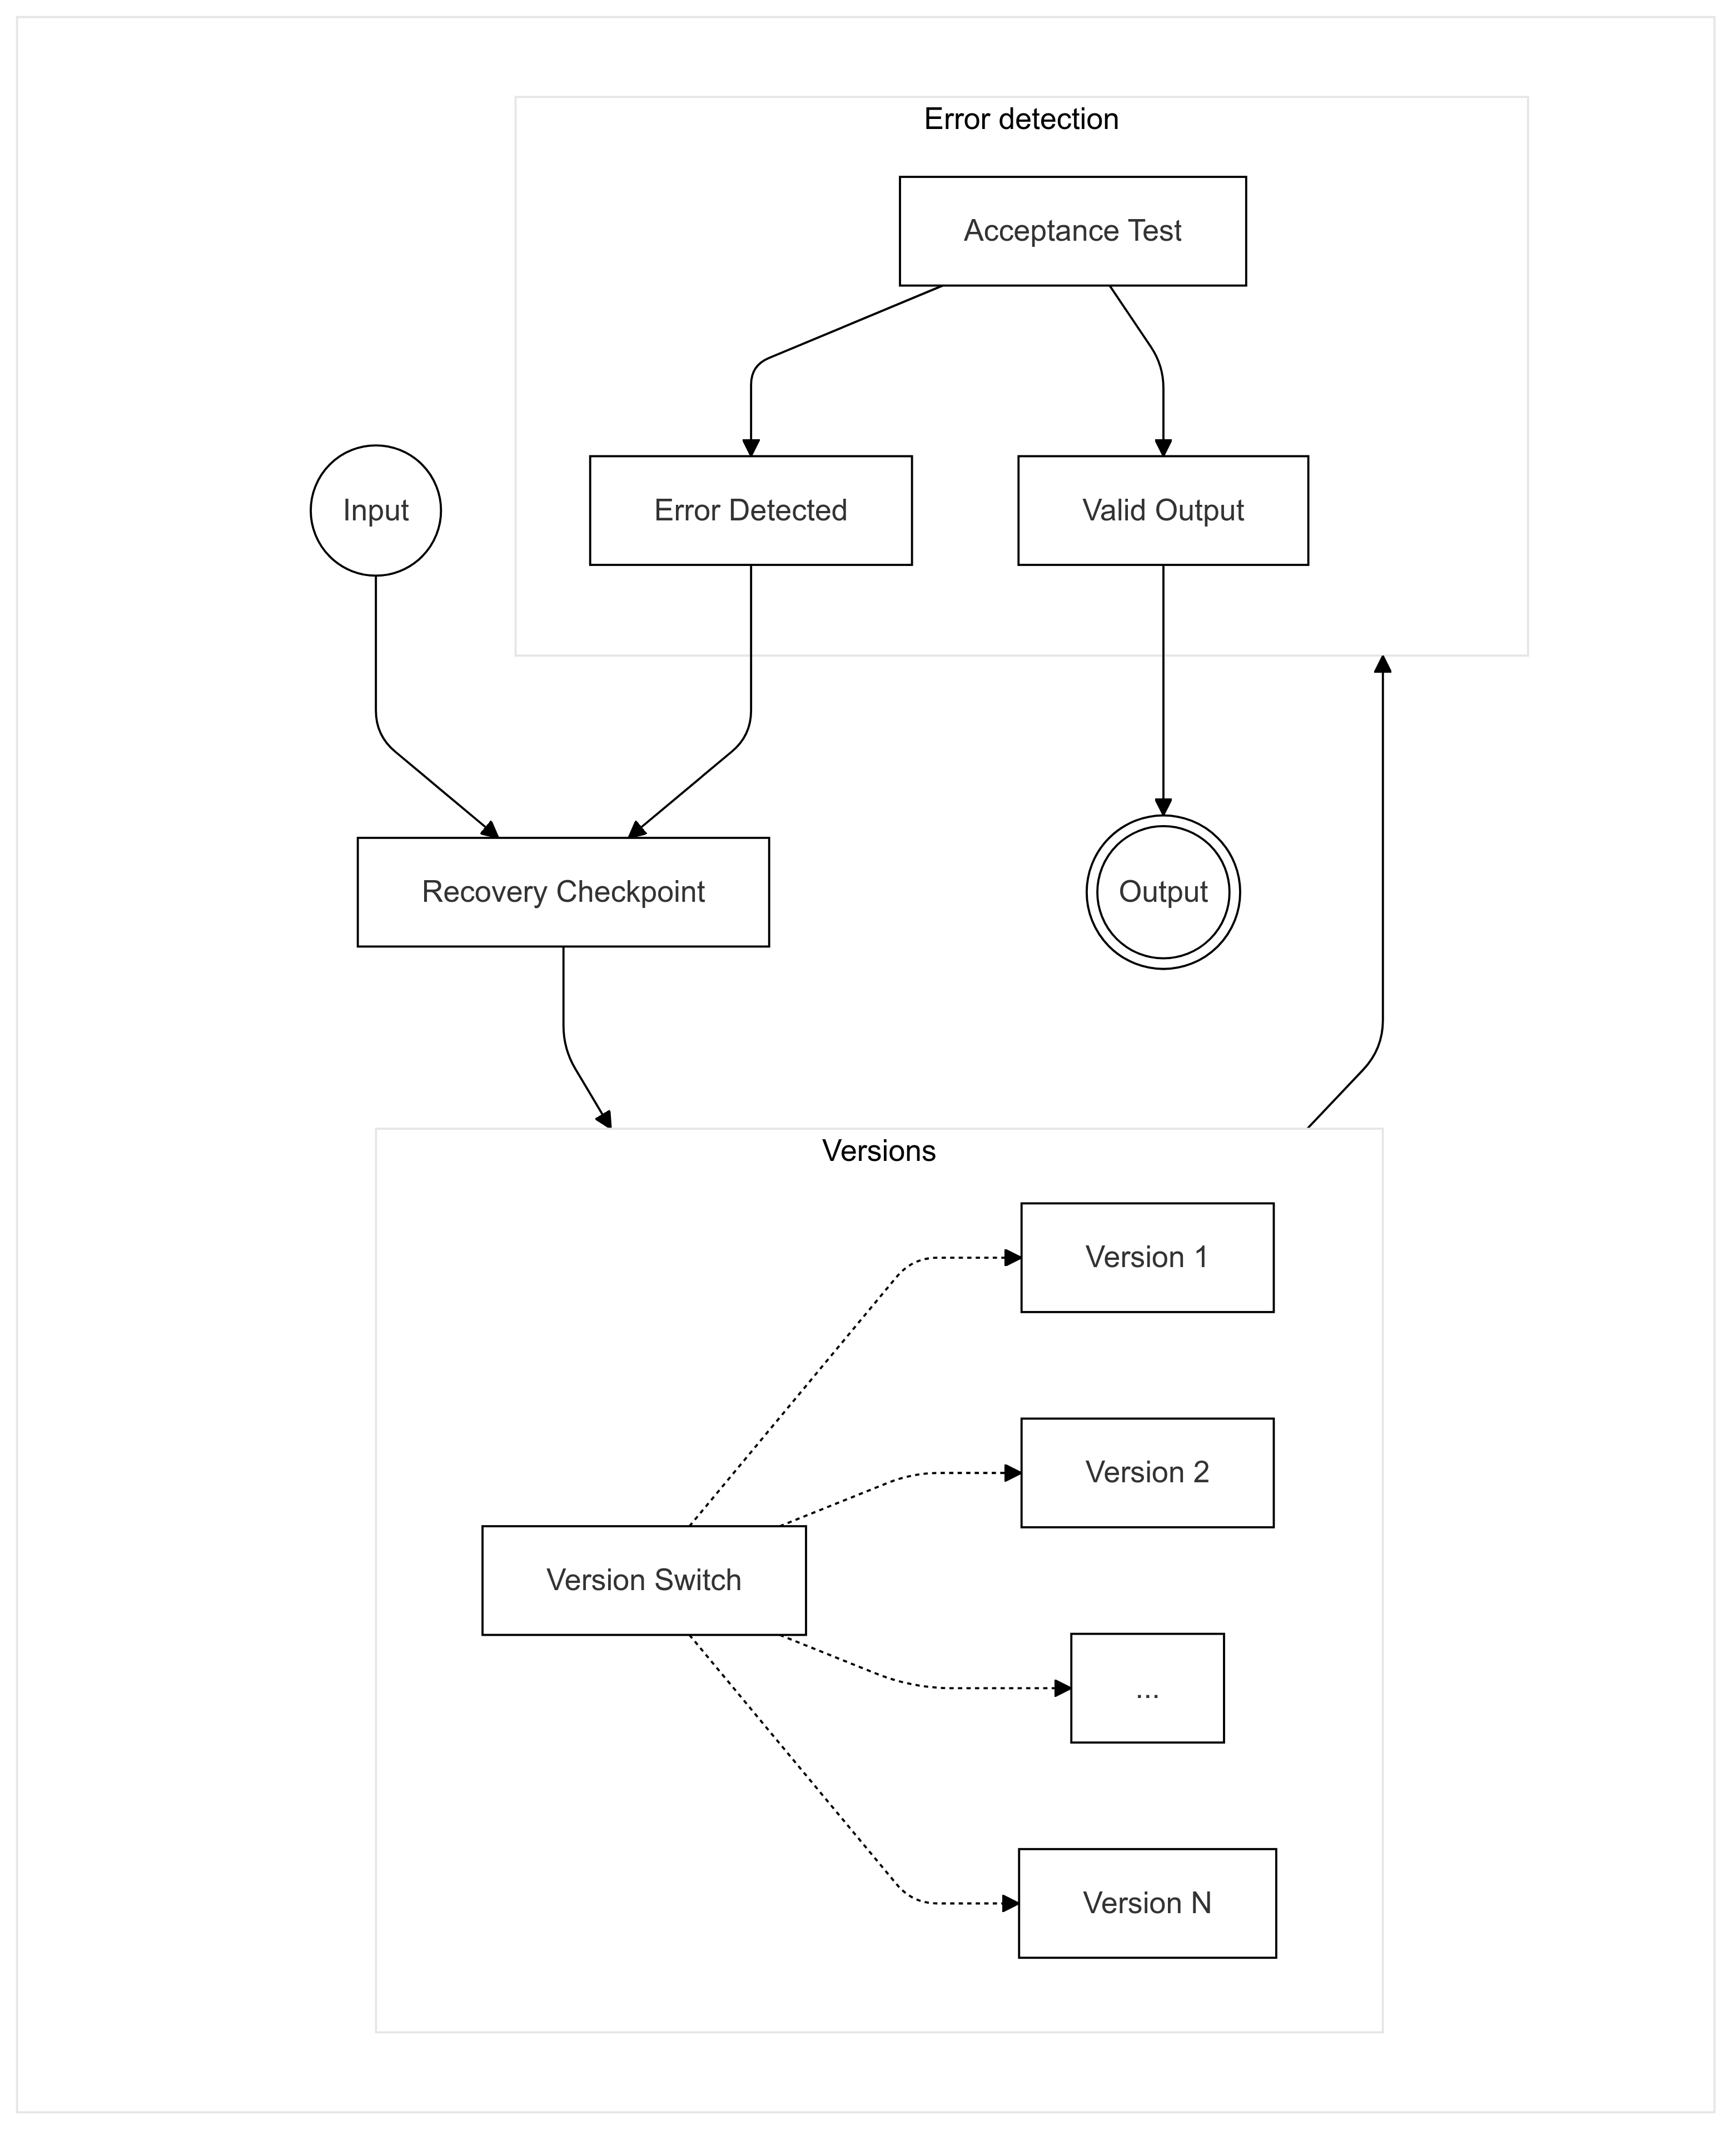
\includegraphics[width=0.9\textwidth]{recovery_blocks/recovery_blocks_01.png}
    \caption{Recovery Blocks}
    \label{fig:rec_blo}
\end{figure}

A key advantage of the recovery blocks technique is that, in most cases, the initial version will execute successfully, allowing subsequent versions to prioritize redundancy and safety over performance. This enables the design of backup versions with gradually reduced performance requirements, ensuring robust fallback options without excessive resource consumption.

Since errors are relatively rare compared to normal execution, this approach often achieves an optimal balance of performance and reliability. By prioritizing efficiency in the primary execution path while incorporating progressively resilient alternatives, recovery blocks can provide dependable fault tolerance without compromising system performance in typical operating conditions. This balance makes recovery blocks a practical solution for systems requiring high availability and reliability.

A considerable drawback of recovery blocks approach is its inherent complexity which creates numerous failure points. Namely during error detection and state recovery. Since we are performing error detection on a singular execution of a version, we have no way to detect errors which coincide with normal functioning of the software, e.g. random bit flips in used variable. Errors such as these would result in incorrect output from a version, but would be undetectable provided the memory corruption is minimal. Even if we do detect an error, we have no guarantee that the state which was saved is not corrupted as well. We would need to employ various techniques to detect a corrupted recovery checkpoint and ideally implement redundancies to ensure the state can be restored.

This creates a lot of overhead and might not be ideal for application where minimal memory footprint is needed.

\subsubsection{N-version programming}

N-version programming extends the multi-version technique by running the same task in parallel across multiple, independent versions, typically referred to as “N versions.” In this approach, each version independently performs the task, and the final outcome is determined through a consensus mechanism that evaluates the results from all N executions.

This consensus is usually achieved through a voting algorithm, which aggregates the outputs from each version and selects the result agreed upon by the majority, thereby reducing the likelihood of errors impacting the system. By leveraging redundancy and voting, N-version programming enhances system reliability and fault tolerance. However, implementing this technique requires careful design to ensure that each version performs equivalently yet independently, minimizing correlated failures and maximizing the robustness of the overall system. Additionally, the increased complexity of maintaining multiple synchronized versions demands significant testing and validation efforts to ensure accurate and efficient performance across all versions.

\begin{figure}[hbt!]
    \centering
    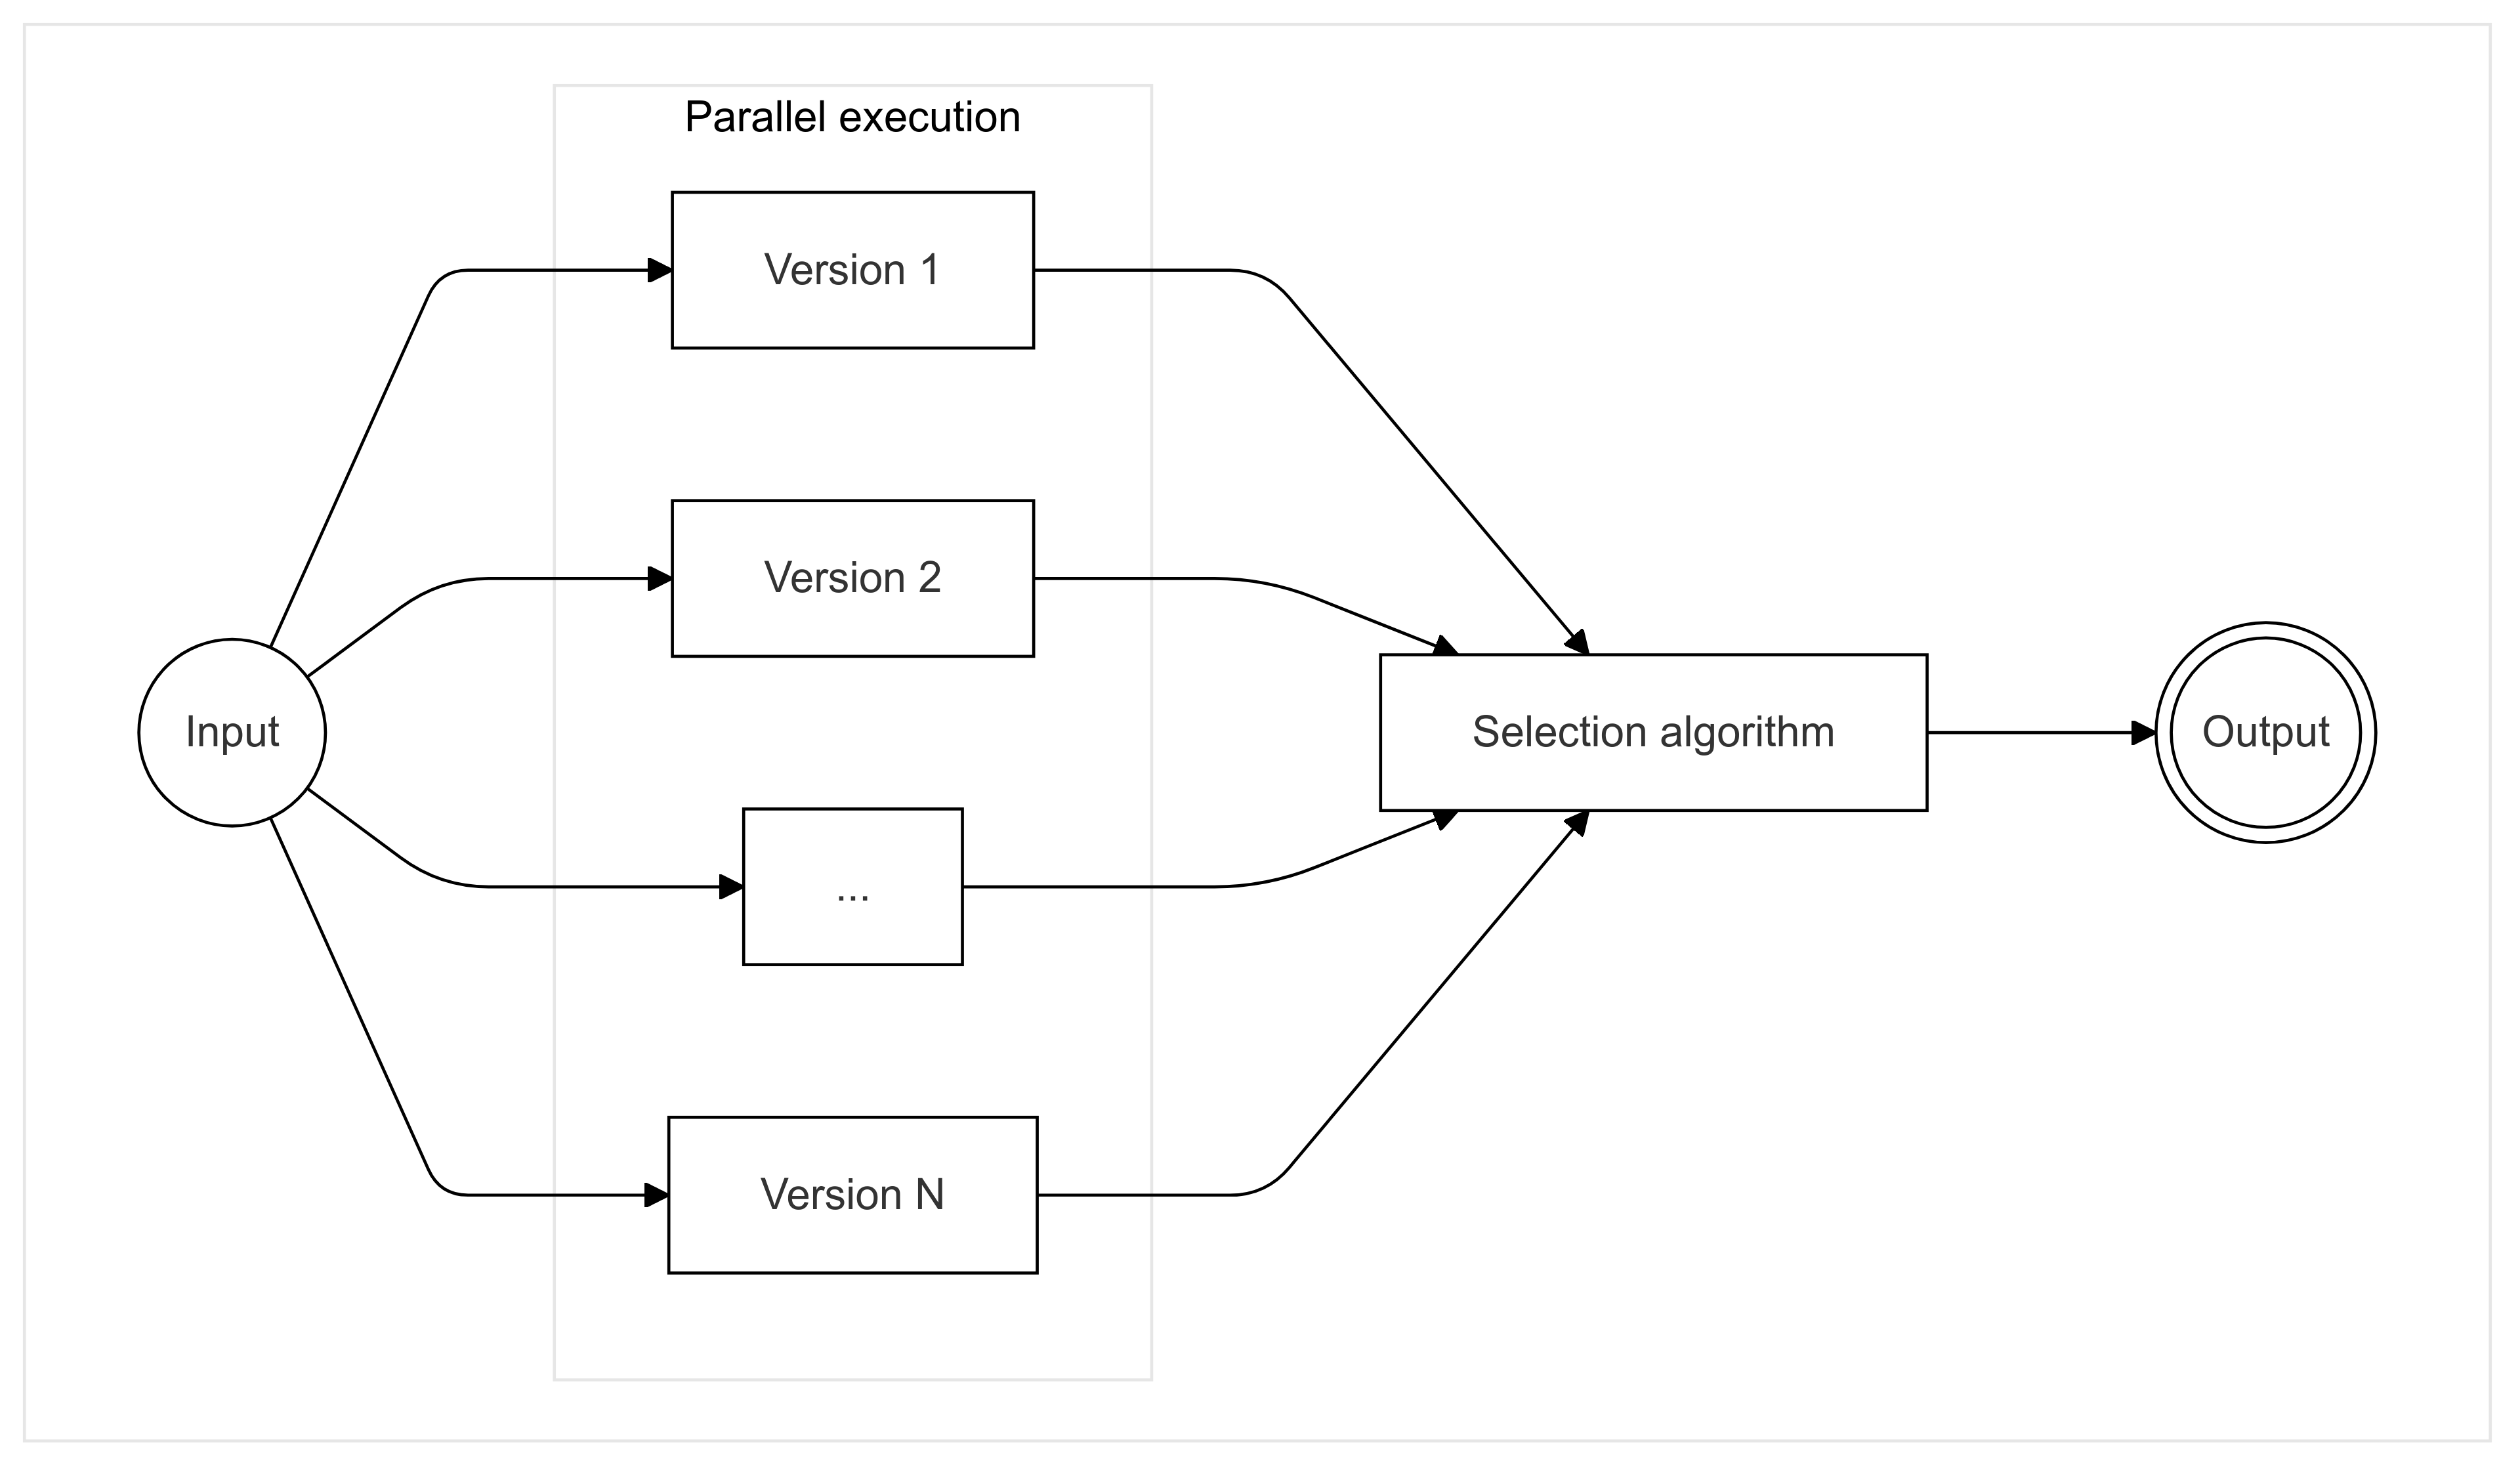
\includegraphics[width=0.9\textwidth]{n_version_prog/n_version_prog.png}
    \caption{N-Version Programming}
\end{figure}

The primary drawback of N-version programming is its requirement to execute all versions either in parallel or sequentially before determining the final output. This can be highly resource-intensive, especially for large or complex tasks, as it necessitates significant computational power and memory to run multiple versions simultaneously.

For systems with limited resources, such as embedded systems, this approach can be particularly inefficient. The need to allocate resources for each version can strain the system’s capabilities, potentially reducing its overall performance and responsiveness. As a result, while N-version programming enhances fault tolerance and reliability, it may not be suitable for applications where resource constraints are a priority or where processing efficiency is critical.

A consideration for N-version programming is the possibility of error not being random indpendent event, but rather a function of the input variable. (https://ieeexplore.ieee.org/document/5326). Therefore, even multiple version running in parallel could all fail and give erroneous results. This makes the selection algorithm a critical failure point which N-version programming on its own does not address.

\subsubsection{N Self-checking programming}

\subsubsection{t/(n-1)-Variant programming}

\subsubsection{Drawbacks of multi-version programming}

The primary challenge associated with multi-version programming is the significant effort required to develop, test, and maintain several versions of software that perform the same function. This process can be resource-intensive, leading to increased costs and inefficiencies that may be prohibitive for smaller projects or for teams with limited budgets.

To achieve effective multi-version programming, each version must be carefully designed to execute the same task while incorporating distinct failure mechanisms. Ensuring that no two versions fail in the exact same way is crucial for building reliable and fault-tolerant systems. This approach allows for enhanced redundancy, as one version can continue to operate even if another encounters a specific failure mode. While this increases the robustness of the system, it also demands rigorous validation to ensure that each version is independently reliable and that the software as a whole remains cohesive across all iterations.

\printbibliography

\end{document}